%%
%% 张哲简历
%%

\documentclass[zh]{resume}

\setmainfont{TeX Gyre Termes}
\setmonofont{Noto Sans Mono}
\setCJKmainfont{Noto Serif CJK SC}

\fileinfo{%
  \faCopyright{} 2026, Zhang Zhe \hspace{0.5em}
  \faEdit{} \today
}

\name{哲}{张}
\makeatletter
\def\@photo@width{2.35cm}
\def\@photo@position{right}
\def\@photo{%
  \begin{minipage}{\@photo@width}
    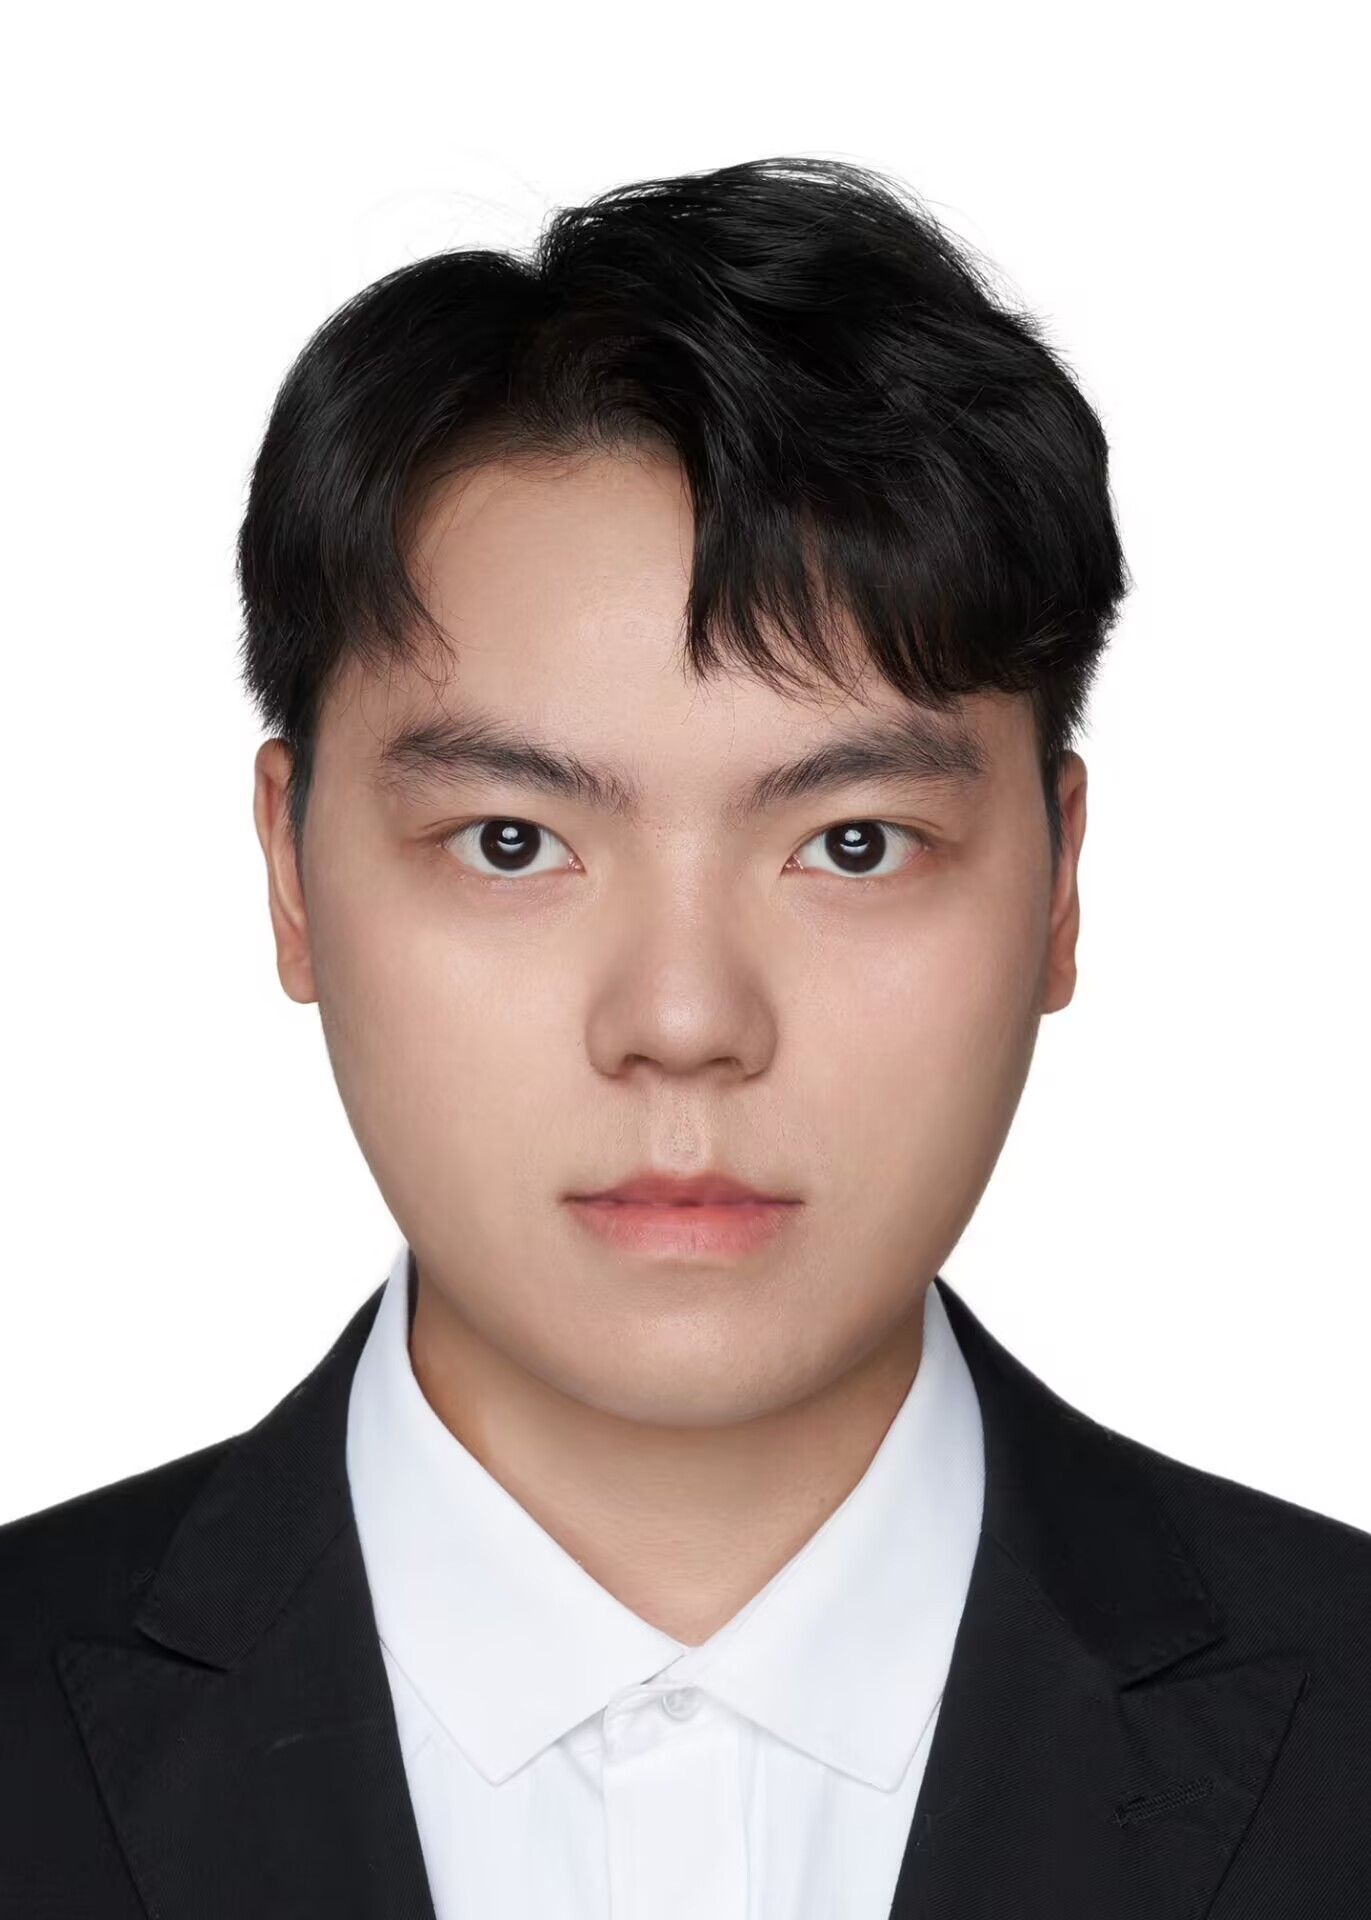
\includegraphics[width=\linewidth]{zhangzhe.jpg}%
  \end{minipage}%
}
\makeatother

\keywords{Agent 开发, LangGraph, MCP, 全栈开发, LLM 应用, 智能运维, Vue3, Node.js}

\profile{
  \mobile{13160006317}
  \email{3220857484@qq.com}
  \university{南京理工大学}
  \degree{软件工程 \textbullet 硕士在读}
}

\begin{document}
\makeheader

\begin{abstract}
南京理工大学软件工程研究生在读，本科毕业于南通大学软件工程专业。具备 Agent 系统设计与全栈工程开发能力，熟悉 LangGraph/LangChain 多智能体编排、MCP 工具协议集成及 LLM 应用落地；主导开发基于 LangGraph 的智能运维诊断 Agent 和教辅录题审核一体化平台，覆盖从 Agent 架构设计、后端服务开发到前端交互的完整链路；同时在 RAG 检索增强、模型微调与强化学习方向有竞赛实践经验。
\end{abstract}

\sectionTitle{教育背景}{\faGraduationCap}
\begin{educations}
  \education%
    {2024.09}%
    [至今]%
    {南京理工大学}%
    {软件工程专业}%
    {软件工程}%
    {硕士}
  \separator{0.5ex}
  \education%
    {2019.09}%
    [2023.06]%
    {南通大学}%
    {软件工程专业}%
    {软件工程}%
    {本科}
\end{educations}

\sectionTitle{比赛经历}{\faTrophy}
\begin{itemize}
  \item \textbf{KDD Cup 2024 学术论文问答检索挑战赛} \hfill 2024.05 -- 2024.07
  \begin{itemize}
    \item \textbf{任务背景}: 面向学术问答场景，从海量论文中检索与专业问题最匹配的候选论文。
    \item \textbf{方案设计}: 针对复杂 Query 冗长、语义匹配难的问题，设计 ``问题精炼 + 向量召回 + 重排序'' 两阶段检索方案；基于 Llama3 对 Query 进行精炼总结，使用 BGE M3 对 Query 与论文语料统一向量化，结合 FAISS 召回 Top100 候选论文，再引入 BGE-Reranker 对结果精排筛选 Top20。
    \item \textbf{优化细节}: 通过 Hard Example Mining 构建微调数据，对 Reranker 进行专项优化，提升困难样本区分能力。
    \item \textbf{结果}: 官方测试集检索分数从 0.138 提升至 0.166，较基线提升约 20.3\%。
  \end{itemize}

  \item \textbf{``天翼云息壤杯'' AI 大赛：大语言模型数学推理能力提升} \hfill 2024.11 -- 2025.07
  \begin{itemize}
    \item \textbf{任务背景}: 基于 Qwen3-8B 开展微调训练，提升模型对复杂数学问题与深度推理的理解求解能力。
    \item \textbf{方案设计}: 围绕数学推理任务长链路推导困难、监督样本质量不足的问题，设计 ``数据蒸馏 + 质量筛选 + 参数高效微调'' 整体方案；基于 MetaMathQA 构建数据集，利用 Qwen2.5-Math-72B 蒸馏生成 10 万条高质量 CoT 样本，并结合 Math-Verify 与 Qwen2.5-72B 评审模型做答案校验。
    \item \textbf{工程落地}: 在 8 卡昇腾 910B 64G 环境完成 Qwen3-8B 的 LoRA 微调，并结合 vLLM 优化推理性能，实现训推一体化部署。
    \item \textbf{结果}: 微调后的 Qwen3-8B 在客观数学题上的正确率从 38\% 提升至 62\%。
  \end{itemize}
\end{itemize}

\sectionTitle{专业技能}{\faCogs}
\begin{itemize}
  \item \textbf{Agent 开发}: 熟悉 LangGraph 状态图编排与多智能体架构设计，掌握条件路由、循环诊断、子图嵌套等复杂工作流构建；熟悉 MCP（Model Context Protocol）工具协议，具备自定义 MCP Server 开发经验。
  \item \textbf{LLM 应用}: 熟悉 LangChain 工具链与 Prompt Engineering，具备 RAG 检索增强（向量召回 + 重排序）、知识蒸馏、LoRA 微调及 GRPO 强化学习实践经验；了解 vLLM 推理部署。
  \item \textbf{后端开发}: 熟悉 Python（FastAPI）和 Node.js（Fastify）后端开发，掌握 PostgreSQL、Redis、BullMQ 消息队列；具备 Prisma ORM、JWT 认证、RESTful API 设计经验。
  \item \textbf{前端开发}: 熟悉 Vue 3 + TypeScript + Vite 技术栈，了解 React/Next.js；掌握 Ant Design Vue、Pinia 状态管理、动态路由等前端工程化实践。
  \item \textbf{DevOps}: 熟悉 Docker/Docker Compose 容器化部署，掌握 Prometheus + Grafana 监控体系搭建，具备 Nginx 反向代理、CI/CD 流程配置经验。
\end{itemize}

\sectionTitle{项目经历}{\faCode}
\begin{itemize}
  \item \textbf{智能运维诊断 Agent（基于 DeerFlow 框架）} \hfill 2026.01 -- 至今
  \begin{itemize}
    \item \textbf{项目背景}: 针对录题审核系统线上告警响应慢、故障定位依赖人工经验的问题，基于字节开源 Agent 框架 DeerFlow，设计并实现一套智能运维诊断 Agent，实现告警自动分类、根因分析与修复建议生成的端到端闭环。
    \item \textbf{Agent 架构}: 基于 LangGraph StateGraph 构建三阶段诊断流水线——Triage（告警分类与严重度评估）$\rightarrow$ Diagnosis（根因分析，置信度 $<$ 0.7 时自动循环深入排查，最多 3 轮）$\rightarrow$ Report（生成结构化诊断报告与修复建议）；通过 DiagnosisState 管理告警类型、指标快照、日志分析、相似案例、置信度等全链路状态。
    \item \textbf{MCP 工具集成}: 开发 3 个自定义 MCP Server 对接生产环境——Prometheus Server（封装 PromQL 查询，提供 CPU/内存/API P95 延迟/队列状态等 8 项预设指标）、Docker Server（容器列表/日志/资源统计，支持白名单隔离）、Logs Server（PostgreSQL 慢查询/Redis 慢查询/Nginx 访问日志的检索与分析）。
    \item \textbf{知识库与评估}: 基于 ChromaDB 构建历史故障案例向量库，支持相似案例检索辅助诊断；设计评估框架，通过 Precision/Recall/F1 和平均置信度量化诊断准确性。
  \end{itemize}

  \item \textbf{教辅录题审核一体化系统} \hfill 2025.06 -- 至今
  \begin{itemize}
    \item \textbf{项目背景}: 面向教辅出版行业，构建覆盖 PDF 教材上传、教师录题、质检抽检、百度教辅系统入库全流程的数字化生产管理平台，替代原有 Excel + 多工具的碎片化工作流。
    \item \textbf{技术架构}: 前端基于 Vue 3 + TypeScript + Ant Design Vue 构建录题工作台（PDF 双栏标注、OCR 识别、公式渲染、草稿自动保存）；后端基于 Fastify + Prisma + PostgreSQL + Redis，采用 BullMQ 持久化队列处理 PDF 拆分、MinerU 内容提取、自动切题等异步任务。
    \item \textbf{自动切题}: 设计 LLM 驱动的自动切题流水线——读取 MinerU 结构化 PDF 内容，按章节页码范围分组，调用大模型提取结构化题目数据；支持分块处理大文档，LLM 失败时自动降级为基于题号索引的规则切题，结果经去重后回填至目录树。
    \item \textbf{运维监控}: 集成 Prometheus + Grafana 监控体系，暴露队列健康、API 延迟、Worker 状态等核心指标；配置告警规则覆盖 P95 延迟、Worker 离线、高 CPU 等场景，为上层运维 Agent 提供数据源。
  \end{itemize}
\end{itemize}

\sectionTitle{科研成果}{\faAtom}
\begin{itemize}
  \item \textbf{QTSF-Net: Quality-aware and Target-guided Weakly Supervised Fusion Network for Multimodal Small Object Detection} \hfill 一作，Under Review
  \begin{itemize}
    \item 针对可见光-红外多模态小目标检测中模态质量失衡、小目标细节丢失和模态缺失鲁棒性不足三大问题，提出 QTSF-Net：设计质量感知跨模态融合模块（QCFM），通过通道级质量评估与空间质量图实现逐通道逐区域的自适应融合；提出目标引导的小目标细节补偿模块（TSDCM），以候选热力图引导 P2 高分辨率特征按需查询，避免全局处理的计算开销；引入模态退化一致性训练策略（MDCTS），结合预测蒸馏与 ROI 级跨模态对比学习增强单模态鲁棒性。
  \end{itemize}
\end{itemize}

\sectionTitle{荣誉奖项}{\faTrophy}
\begin{itemize}
  \item WACV 2025 目标距离估计挑战赛，国家级冠军
  \item ICCV 2025 感知测试挑战赛：多项选择题视频问答，国家级冠军
  \item ``天翼云息壤杯'' 高校 AI 大模型比赛（华为）国家级三等奖
  \item CVPR 2025 少样本目标检测，国家级三等奖
\end{itemize}

\end{document}
